\documentclass[]{article}

\usepackage[utf8]{inputenc}
\usepackage[T1]{fontenc}

\usepackage{amsmath}
\usepackage{color}
\usepackage{hyperref}
\usepackage{graphicx}
\usepackage{listings}
\usepackage{lstautogobble}
\usepackage{svgcolor}
\setlength{\parindent}{0cm}

\definecolor{MediumBlue}{rgb}{0.000,0.000,0.804}
\definecolor{DarkGreen}{rgb}{0.000,0.392,0.000}

% Settings for lstlistings
\lstset{%
  basicstyle=\ttfamily,
  columns=fullflexible,
  autogobble,
  keywordstyle=\bfseries\color{MediumBlue},
  stringstyle=\color{DarkGreen},
  commentstyle=\itshape\color{gray},
  tabsize=4
}

%% Listings definition for D programming language
%% Author : Jesse Phillips <Jesse.K.Phillips+D@gmail.com>

\lstdefinelanguage{D}{
  % Keywords
  morekeywords=[1]{
    abstract, alias, align, assert, auto, body, break, cast, catch, class, const,
	 continue, debug, delegate, delete, deprecated, do, else, enum, export,
	 false, final, finally, for, foreach, foreach_reverse, function, goto, if,
	 immutable, import, in, inout, interface, invariant, is, lazy, macro, mixin,
	 module, new, nothrow, null, out, override, package, pragma, private,
	 protected, public, pure, ref, return, shared, static, struct, super,
	 switch, synchronized, template, this, throw, true, try, typedef, typeid,
	 typeof, union, unittest, volatile, while, with
},
  % Special identifiers, common functions
  morekeywords=[2]{enforce},
  % Ugly identifiers
  morekeywords=[3]{
    __DATE__, __EOF__, __FILE__, __LINE__, __TIMESTAMP__, __TIME__, __VENDOR__,
    __VERSION__, __ctfe, __gshared, __monitor, __thread, __vptr, _argptr,
    _arguments, _ctor, _dtor
},
  % Basic types
  morekeywords=[4]{
	 byte, ubyte, short, ushort, int, uint, long, ulong, cent, ucent, void,
	 bool, bit, float, double, real, ushort, int, uint, long, ulong, float,
	 char, wchar, dchar, string, wstring, dstring, ireal, ifloat, idouble,
	 creal, cfloat, cdouble, size_t, ptrdiff_t, sizediff_t, equals_t, hash_t
},
  % Strings
  morestring=[b]{"},
  morestring=[b]{'},
  morestring=[b]{`},
  % Comments
  comment=[l]{//},
  morecomment=[s]{/*}{*/},
  morecomment=[s][\color{blue}]{/**}{*/},
  morecomment=[n]{/+}{+/},
  morecomment=[n][\color{blue}]{/++}{+/},
  % Options
  sensitive=true
}



% Title Page
\title{Supplementary material for the transformed density rejection algorithm}
\author{}


\begin{document}
\maketitle

\begin{abstract}
This document aims to provide an understandable guide to the transformed density rejection algorithm and explain all choices made for the mir implementation.
\end{abstract}

\section{Intro to random sampling}

The \href{https://github.com/libmir/mir/pull/240}{code} is currently WIP and will be available at \texttt{mir.random.flex}. The report \textit{Transformed Density Rejection with Inflection Points} can be found  \href{http://epub.wu.ac.at/3158/1/techreport-110.pdf}{here}.

\subsection{The problem}

Given a uniform random generator, sample non-uniform random values.

\subsection{The inversion method}

The underlying idea of random sampling is that given an inverse function $F^{-1}$ for the cumulative density function (CDF), we map random values to a distribution. Given $F^{-1}$ values from the density can be sampled by using the given uniform random generator.
For example for the exponential distribution sampling would be:

\begin{lstlisting}[language=D]
S sample(S, RNG, FInv)(RNG gen, FInv finv)
{
    import std.random : uniform;
    S u = uniform!("[]", S)(0, 1);
    return finv(u);
}
import std.random : rndGen;
auto fInvExp = (S x) => -log(S(1) - x);
sample(rndGen, fInvExp)
\end{lstlisting}

However there are two big problems: (1) for most densities the inverse CDF is not known or can't be determined or (2) if it can be determined it's usually very computationally expensive function (e.g. iterative numeric approximation needs to be used if no exact form can be found).

\subsection{The rejection method}

An very popular alternative is the \textit{rejection} method - often known as \textit{acceptance-rejection} sampling. It only requires one to know the density of a distribution. The general idea is that if a random variable $(x, y)$ is distributed within the density $f$, then it has the density $f$.

If we have a function $h(x)$ that majorizes the density function $f(x)$ (in this simple example $x = 1$) - in other words $ \forall x \in [l, r]: f(x) < h(x)$ where $l$ and $r$ are the left and right boundaries of an interval - then we use the hat function.

 can define $f(x) / h(x)$. Note that this is typically written with a constant $M$: $h'(x) = M * h(x))$. 

1) We sample a point from the area of our majorizing hat function (=linear)


This means we can simplify sample $x$ and $y$ uniformly and check whether the generated point is in the area covered by the density function. If it's within the area the point is \textit{accepted}, otherwise it is \textit{rejected} and new points are sampled until a point that is within the area and thus can be accepted is drawn.

\begin{figure}[h!]
\centering
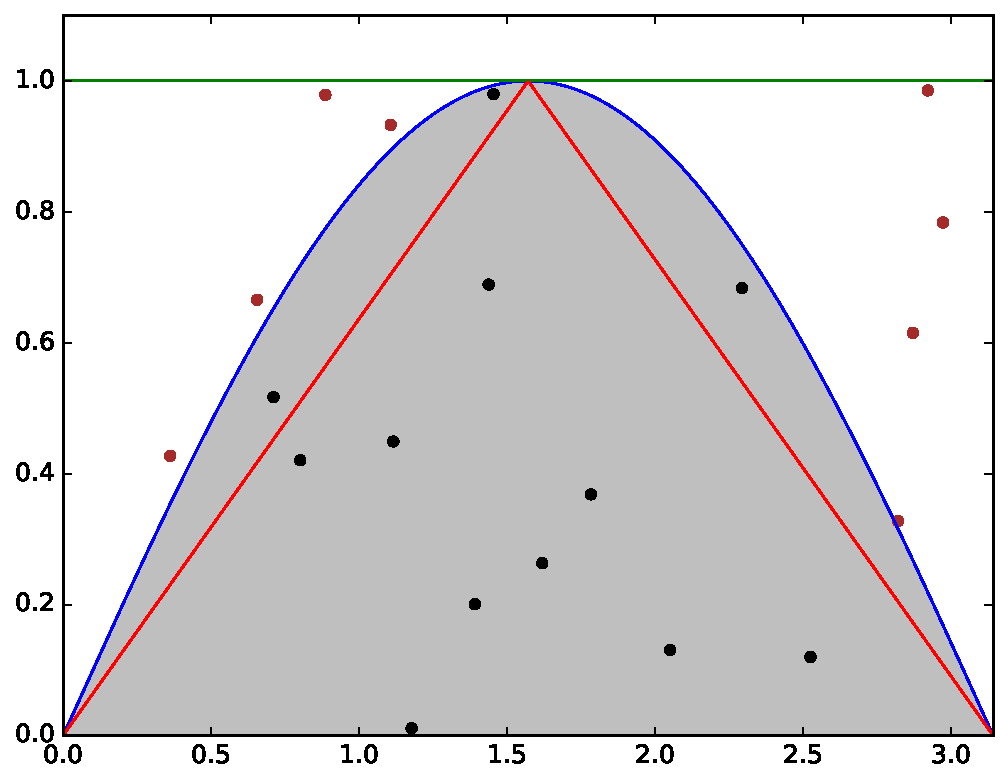
\includegraphics[width=0.8\textwidth]{figs/rejection_sampling.pdf}
\caption{Rejection sampling of $sin(x)$ (blue). Hat function (green), squeeze function in red. Points are marked black when accepted, and brown for rejected.}
\label{fig:rejection_method}
\end{figure}

A simplified example of the basic rejection method can be seen here:

\begin{lstlisting}[language=D]
S sample(S, RNG, Pdf, Hat)(RNG gen, Pdf pdf, Hat hat, S left, S right)
{
    import std.random : uniform;
    for (;;)
    {
        // generate x with density proportional to hat(x)
        S x = uniform!("[]", S)(left, right, gen);
        S y = uniform!("[]", S)(0, 1, gen);
        // check whether the sampled point is within the density
        if (y * hat(x) <= pdf(x))
            return x;
    }
}
import std.math : PI, sin;
import std.random: rndGen;
sample(rndGen, (S) => sin(x), (S x) => 1, 0, PI);
\end{lstlisting}

Furthermore the performance of this method depends heavily on the ratio of $f(x) / h(x) = 1 / \rho$, where $\rho$ is the average number of needed iterations to sample one value.

\subsubsection{Rejection with inversion}

Just a straight line as upper bound yields a lot of uncovered areas, thus we want to use more generic \textit{hat} functions:

\begin{lstlisting}[language=D]
S sample(S, RNG, Pdf, Hat)(RNG gen, Pdf pdf, Hat hat, Hat hatInvCDF)
{
    import std.random : uniform;
    for (;;)
    {
        S u = uniform!("[]", S)(0, 1, gen);
        // generate x with density proportional to hat(x)
        S x = hatInvCDF(u);
        S y = uniform!("[]", S)(0, 1, gen);
        // check whether the sampled point is within the density
        if (y * hat(x) <= pdf(x))
            return x;
    }
}
import std.math : PI, sin;
import std.random: rndGen;
auto hatInvCDF = (S u) => 0 + u * (PI - 0);
auto hat = (S x) => 1;
sample(rndGen, (S) => sin(x), hat, hatInvCDF 0, PI);
\end{lstlisting}

The (Tin)flex algorithm will show a way to automatically construct a hat function for any differentiable density function.

\section{Intro to (Tin)flex}

\subsection{Transformations}

Tinflex uses a family of transformation of the pdf function. They can be grouped in two classes:

\subsubsection{$c \neq 0$}

%The general transformation function is $x^c$, however as it's only defined in $\mathbb{C}$, we need to restrict it to positive numbers.

\[T_c(x) = sgn(c) * x^c\]

With the usual inversion rules we get

\begin{align*}
y &= sgn(c) * x^c \\
log(y) &= log(sgn(c)) + log(x^c) \\
log(y) &= log(sgn(c)) + c * log(x) \\
\frac{log(y) - log(sgn(c))}{c} &= log(x) \\
exp\left(\frac{log(y) - log(sgn(c))}{c}\right) &= x
\end{align*}

and it's inverse:

\[T_c^{-1}(x) = sgn(c) * (sgn(c) * x)^{\frac{1}{c}}\]


\begin{figure}[p]
\centering
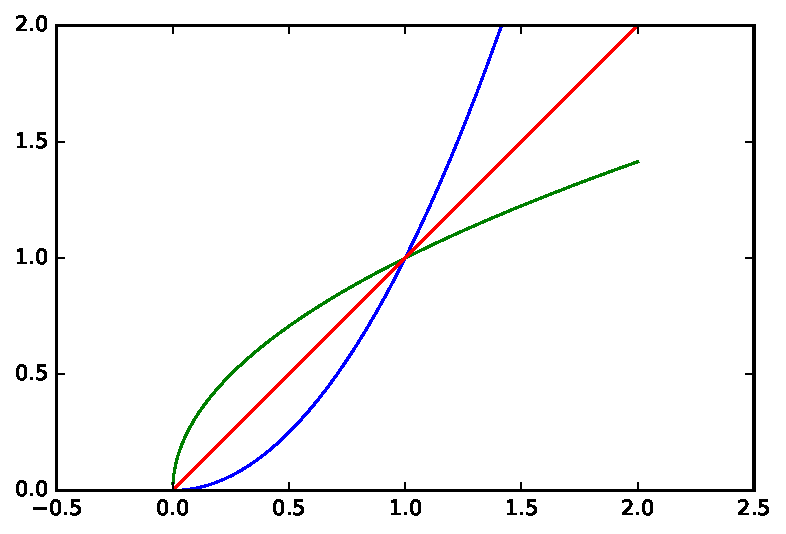
\includegraphics[width=0.8\textwidth]{figs/a_2_sgn_pow.pdf}
\caption{Exponential function (red) and it's inverse the natural log (blue)}
\label{fig:log_exp}
\end{figure}

\subsubsection{$c = 0$}

\[T_c(x) = log(x)  \]

and it's inverse:

\[T_c^{-1}(x) = exp(x) \]


\begin{figure}[p]
\centering
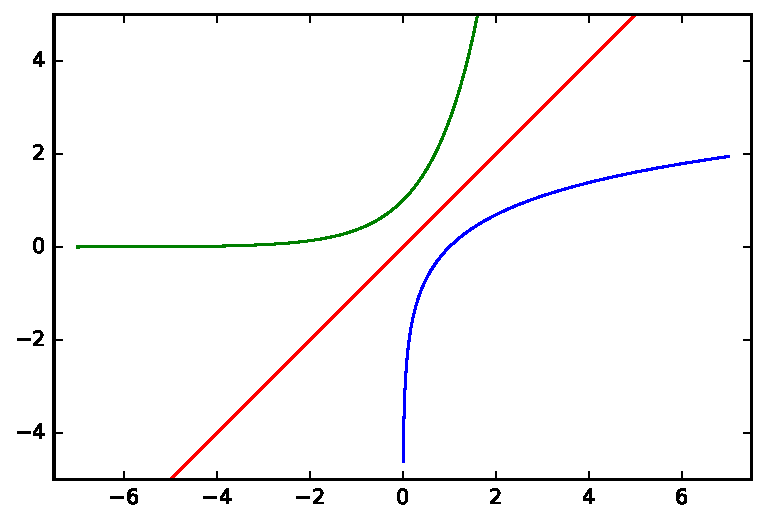
\includegraphics[width=0.8\textwidth]{figs/log_exp}
\caption{Exponential function (red) and it's inverse the natural log (blue)}
\label{fig:log_exp}
\end{figure}

\ \\

Please note in the Tinflex paper and below this case is split into multiple common cases to have simpler formulas and reduce numerical errors.

Moreover according to the paper $f(x)$ is the pdf, and $\tilde{f}(x)$ is its transformation.

\[\tilde{f}(x) = T_c(f(x))  \]

\subsubsection{Input of Tinflex}

Tinflex expects the \textbf{log}-density, which means that for $c = 0$, no transformations need to be applied.
However for $c \neq 0$ the inverse is needed, we first needs to apply the \textit{inverse} $T_c^{-1}(x) = exp(x)$ and then apply the other $T_c$ transformation:

\begin{align*}
\tilde{f}(x) &= exp(T_{c \neq 0}(x)) \\
&= exp(sgn(c) * x^c) \\
&= sgn(c) * exp(x * c)
\end{align*}

\subsection{Linear functions}

The Tinflex paper uses the following definition for linear functions which are used in parts to construct hat and squeeze functions. The hat function majorizes the \textit{transformed} pdf, whereas the \textit{transformed} pdf majorizes the squeeze function.

\[ \tilde{f}(x) = \alpha + \beta * (x - x_0) \]

In the latter $h(x)$ will also be used instead of $\tilde{f}(x)$.
Remember that the transformation is applied with $T_c(x)$.

\subsection{Construction of linear functions}

For both secants and tangents $x_0$ and $\alpha$ are defined as follows:

\begin{enumerate}
\item $x_0$ is $b_l$ if $\tilde{f}(b_l) >= \tilde{f}(b_r)$, $b_r$ otherwise
\item $\alpha = \tilde{f}(x_0)$
\end{enumerate}

In fact only $\beta$ is defined differently: \\ 
\ \\
Tangent: $\beta = \tilde{f}'(x_0)$ \\ 
Secant:  $\beta = \frac{\tilde{f}(b_r) - \tilde{f}(b_l)}{b_r - b_l}$


\section{Area $A_h$}

\begin{align*}
A_h &= \int_{b_l}^{b_r} h(x) dx \\
&= \int_{b_l}^{b_r} T^{-1}(\alpha + \beta * (x - x_0)) dx \\
&= \frac{1}{\beta} \big( F_T (\alpha + \beta * (b_r - x_0)) - F_T(\alpha + \beta * (b_l - x_0)) \big) \\
&= \frac{1}{\beta} \big( F_T (h(b_r)) - F_T(h(b_l)) \big)
\end{align*}

\textcolor{red}{TODO: explain why the $\frac{1}{\beta}$ appears here}

\subsection{c = 1}

 $F_T = \frac{1}{2} * x^{\frac{2}{1}}$:

\begin{align*}
A_h &= \frac{1}{\beta} \big(h(b_r) - h(b_l) \big) \\
&= \frac{1}{\beta} \left(0.5 * (\alpha + \beta * (b_r - x_0))^2 - 0.5 * (\alpha + \beta * (b_l - x_0))^2 \right) \\
\end{align*}

\subsubsection{Z-Trick}

Z-Trick, $x_0$ can only be either $b_r$ or $b_l$, thus either $b_r - x_0$ or $b_l - x_0$ is zero. \\

\textbf{$I) \quad x_0 = b_l$}

\begin{align*}
A_h &= \frac{0.5}{\beta} \left( (\alpha + \beta * (b_r - b_l))^2 - \alpha^2  \right) \\
&= \frac{0.5}{\beta} \left( \alpha^2 + 2 * \alpha * \beta * (b_r - b_l) + (\beta * (b_r - b_l))^2 - \alpha^2  \right) \\
&= \frac{0.5}{\beta} \left( 2 * \alpha * \beta * (b_r - b_l) + (\beta * (b_r - b_l))^2 \right) \\
&= 0.5 * \left( 2 * \alpha * (b_r - b_l) + \beta * (b_r - b_l)^2 \right) \\
&= 0.5 * (b_r - b_l) * \left( 2 * \alpha  + \beta * (b_r - b_l) \right) \\
&= (b_r - b_l) * \left(\alpha  + 0.5 * \beta * (b_r - b_l) \right) \\
\end{align*}

\textbf{$II) \quad x_0 = b_r$}

\begin{align*}
A_h &= \frac{0.5}{\beta} \left( \alpha^2 - (\alpha + \beta * (b_l - b_r))^2 \right) \\
&= \frac{0.5}{\beta} \left( \alpha^2 - \alpha^2 - 2 * \alpha * \beta * (b_l - b_r) - (\beta * (b_l - b_r))^2   \right) \\
&= \frac{0.5}{\beta} \left( - 2 * \alpha * \beta * (b_l - b_r) - (\beta * (b_l - b_r))^2 \right) \\
&= -0.5 * \left( 2 * \alpha * (b_l - b_r) + \beta * (b_l - b_r)^2 \right) \\
&= -0.5 * (b_l - b_r) * \left( 2 * \alpha  + \beta * (b_l - b_r) \right) \\
\end{align*}

\textcolor{red}{Current code is different}

\subsection{c = 0}

$F_T = e^x$

\begin{align*}
A_h &= \frac{1}{\beta} \left( e^{h(b_r)} - e^{h(b_l)} \right)
\end{align*}

\textcolor{green}{Similar to current code.}

Z-trick:

I) $x_0 = b_l$:

\begin{align*}
A_h &= \frac{1}{\beta} \left( e^{h(b_r)} - e^{h(b_l)} \right) \\
&= \frac{1}{\beta} \left( e^{\alpha + \beta * (b_r - x_0)} - e^{\alpha + \beta * (b_r - x_0)} \right) \\
&= \frac{1}{\beta} \left( e^{\alpha + \beta * (b_r - b_l)} - e^{\alpha} \right) \\
&=\frac{e^{\alpha}}{\beta} \left( e^{\beta (b_r - b_l)} - 1 \right) \\
\end{align*}

where $e^{\alpha} = g(x)$

Approximation with Taylor-Series of $n = 4$ with $k = \beta (b_r - b_l)$

\begin{align*}
A_h &= \frac{e^{\alpha}}{\beta} \left(1 + k + \frac{k^2}{2} +  \frac{k^3}{6} + \frac{k^4}{24} - 1 \right)
\end{align*}

II) $x_0 = b_r$:

\begin{align*}
A_h &=\frac{e^{\alpha}}{\beta} \left(1 - e^{\beta (b_l - b_r)}\right) \\
\end{align*}

with Taylor

\begin{align*}
A_h &= \frac{e^{\alpha}}{\beta} \left(1 - \left(1 + k + \frac{k^2}{2} +  \frac{k^3}{6} + \frac{k^4}{24} \right) \right)
\end{align*}

\textcolor{red}{Different to current code.}

\subsection{c = -0.5}

$F_T = \frac{1}{x^2}$

\begin{align*}
A_h &= \frac{1}{\beta} \left(\frac{1}{h(b_r)^2} - \frac{-1}{h(b_l)^2} \right) \\
& = \frac{1}{\beta} \left(\frac{1}{h(b_r)^2} - \frac{1}{h(b_l)^2} \right)
\end{align*}

\subsubsection{Z-trick}


$F_T = - \frac{1}{x}$

\begin{align*}
A_h &= \frac{1}{\beta} \left(\frac{-1}{h(b_r)} - \frac{-1}{h(b_l)} \right) \\
& = \frac{1}{\beta} \left(- \frac{1}{h(b_r)} + \frac{1}{h(b_l)} \right)
\end{align*}

\subsubsection{Z-trick}

I)

\begin{align*}
A_h & = \frac{1}{\beta} \left(- \frac{1}{\alpha - (\beta * (b_l - b_r)} + \frac{1}{\alpha} \right)
\end{align*}

II)

\begin{align*}
A_h & = \frac{1}{\beta} \left(- \frac{1}{\alpha} + \frac{1}{\alpha - (\beta * (b_r - b_l)} \right)
\end{align*}

\textcolor{red}{Different to current code}

\subsection{c = -1}

$F_T = - log(-x)$

\begin{align*}
A_h &= \frac{1}{\beta} \left(-log(-h(b_r)) + log(-(h_l)) \right) \\
&= \frac{1}{\beta} \left(-log(-\alpha - (\beta * (b_r - b_l))) + log(-\alpha) \right)
\end{align*}

\subsubsection{Z-trick}

I) $x_0 = b_l$

\begin{align*}
A_h &= \frac{1}{\beta} \left(-log(-h(b_r)) + log(-(h_l)) \right) \\
&= \frac{1}{\beta} \left(-log(-\alpha - (\beta * (b_r - b_l))) + log(-\alpha) \right)
\end{align*}

II) $x_0 = b_r$

\begin{align*}
A_h &= \frac{1}{\beta} \left(- log(-\alpha) + log(-\alpha - (\beta * (b_r - b_l))) \right)
\end{align*}

\subsection{$c > 0$}

$F_T = \frac{c}{c + 1} * x^{\frac{c + 1}{c}}$

\begin{align*}
A_h &= \frac{1}{\beta} \left( \frac{c}{c + 1} h(b_r)^{\frac{c + 1}{c}} - \frac{c}{c + 1} h(b_l)^{\frac{c + 1}{c}} \right) \\
A_h &= \frac{c}{\beta * (c + 1)}  \left( h(b_r)^{\frac{c + 1}{c}} - h(b_l)^{\frac{c + 1}{c}} \right) \\
\end{align*}

I) $x_0 = b_l$

\begin{align*}
A_h &= \frac{c}{\beta * (c + 1)}  \left( (\alpha + \beta * (b_r - b_l))^{\frac{c + 1}{c}} - (\alpha)^{\frac{c + 1}{c}} \right) \\
\end{align*}

II) $x_0 = b_r$

\begin{align*}
A_h &= \frac{c}{\beta * (c + 1)}  \left( (\alpha)^{\frac{c + 1}{c}} - (\alpha + \beta * (b_l - b_r))^{\frac{c + 1}{c}} \right) \\
\end{align*}

\subsection{$c < 0$}

$F_T = - \frac{c}{c + 1} * (-x)^{\frac{c + 1}{c}}$

\begin{align*}
A_h &= \frac{1}{\beta} \left( - \frac{c}{c + 1} (-h(b_r))^{\frac{c + 1}{c}} + \frac{c}{c + 1} (-h(b_l))^{\frac{c + 1}{c}} \right) \\
A_h &= \frac{c}{\beta * (c + 1)}  \left( - (-h(b_r))^{\frac{c + 1}{c}} + (-h(b_l))^{\frac{c + 1}{c}} \right) \\
\end{align*}

I) $x_0 = b_l$

\begin{align*}
A_h &= \frac{c}{\beta * (c + 1)}  \left( - (- \alpha - \beta * (b_r - b_l))^{\frac{c + 1}{c}} + (-\alpha)^{\frac{c + 1}{c}} \right) \\
\end{align*}

II) $x_0 = b_r$

\begin{align*}
A_h &= \frac{c}{\beta * (c + 1)}  \left(- (-\alpha)^{\frac{c + 1}{c}} + (- \alpha - \beta * (b_r - b_l))^{\frac{c + 1}{c}}\right) \\
\end{align*}

\section{Inversion}

$H(b_r) = A(b_r)$ and then $h(x) = h(b_l)$

\begin{align*}
H(x) &= \frac{1}{\beta} \big( F_T (h(x)) - F_T(h(a)) \big)
\end{align*}

then if $H(x) = U$:

\begin{align*}
U &= \frac{1}{\beta} \big( F_T (h(x)) - F_T(h(a)) \big) \\
U * \beta &=\big( F_T (h(x)) - F_T(h(a)) \big) \\
(U * \beta) + F_T(h(a)) &= F_T (h(x)) \\
F_T^{-1} ( (U * \beta) + F_T(h(a))) &= F_T^{-1}( F_T (h(x))) \\
 &= h(x) \\
h^{-1} \left( F_T^{-1} ( (U * \beta) + F_T(h(a))) \right) &= x \\
x_0 + \frac{1}{\beta} \left( F_T^{-1} ( (U * \beta) + F_T(h(a))) - \alpha \right) &= x
\end{align*}

as $h(x) = \alpha + \beta * (x - x_0)$ and thus 

\begin{align*}
y &= \alpha + \beta * (x - x_0) \\
y - \alpha &= (x - x_0) \\
\frac{y - \alpha}{\beta} &=  (x - x_0) \\
x_0 + \frac{y - \alpha}{\beta} &=  x \\
\end{align*}

\subsection{c = 0}

$F_T = e^x$, $F_T^{-1} = log(x)$

\begin{align*}
H^{-1}(U) &= h^{-1} \left( log \left( U\beta + e^{h(a)} \right) \right) \\
\end{align*}

\textcolor{green}{similar to current code.}

\subsection{c = 1}

$F_T = 0.5 * x^2$, $F_T^{-1} = (2x)^{0.5}$

\begin{align*}
H^{-1}(U) &= h^{-1} \left( 2 * \left( U\beta + (0.5 *h(a))^{2} \right) \right)^{0.5} \\
\end{align*}

\subsection{c = -0.5}

$F_T = -\frac{1}{x}$, $F_T^{-1} = - \frac{1}{x}$

\begin{align*}
H^{-1}(U) &= h^{-1} \left( - \frac{1}{U\beta - \frac{1}{h(a)}} \right) \\
\end{align*}


\subsection{c = -1}

$F_T =-log(-x)$, $F_T^{-1} = -exp(-x)$

\begin{align*}
H^{-1}(U) &= h^{-1} \left( - exp \left( U\beta - log(-h(a)) \right) \right) \\
\end{align*}


\subsection{$c > 0$}

$F_T = \frac{c}{c + 1} * x^{\frac{c + 1}{c}}$,
$F_T^{-1} = \frac{c + 1}{c} * x^{\frac{c}{c + 1}}$


\begin{align*}
H^{-1}(U) &= h^{-1} * \frac{c + 1}{c} * \left( U\beta + \frac{c}{c + 1} * (h(a))^{\frac{c + 1}{c}} \right)^{\frac{c}{c + 1}} \\
\end{align*}

\subsection{$c < 0$}

$F_T = - \frac{c}{c + 1} * (-x)^{\frac{c + 1}{c}}$,
$F_T^{-1} = - \frac{c + 1}{c} * (-x)^{\frac{c}{c + 1}}$


\begin{align*}
H^{-1}(U) &= h^{-1} * - \frac{c + 1}{c} * \left(- U\beta - \frac{c}{c + 1} * - (-h(a))^{\frac{c + 1}{c}} \right)^{\frac{c}{c + 1}} \\
&= h^{-1} * - \frac{c + 1}{c} * \left(- U\beta + \frac{c}{c + 1} (-h(a))^{\frac{c + 1}{c}} \right)^{\frac{c}{c + 1}} \\
\end{align*}


\end{document}          